%%%%%%%%%%%%%%%%%%%%%%%%%%%%%%%%%%%%%%%%%%%%%%%%%%%%%%%%%%%%%%%%%%%%
%% I, the copyright holder of this work, release this work into the
%% public domain. This applies worldwide. In some countries this may
%% not be legally possible; if so: I grant anyone the right to use
%% this work for any purpose, without any conditions, unless such
%% conditions are required by law.
%%%%%%%%%%%%%%%%%%%%%%%%%%%%%%%%%%%%%%%%%%%%%%%%%%%%%%%%%%%%%%%%%%%%

\documentclass[
  digital, %% This option enables the default options for the
           %% digital version of a document. Replace with `printed`
           %% to enable the default options for the printed version
           %% of a document.
  oneside, %% This option enables double-sided typesetting. Use at
           %% least 120 g/m² paper to prevent show-through. Replace
           %% with `oneside` to use one-sided typesetting; use only
           %% if you don’t have access to a double-sided printer,
           %% or if one-sided typesetting is a formal requirement
           %% at your faculty.
  table,   %% This option causes the coloring of tables. Replace
           %% with `notable` to restore plain LaTeX tables.
  lof,     %% This option prints the List of Figures. Replace with
           %% `nolof` to hide the List of Figures.
  nolot,     %% This option prints the List of Tables. Replace with
           %% `nolot` to hide the List of Tables.
  %% More options are listed in the user guide at
  %% <http://mirrors.ctan.org/macros/latex/contrib/fithesis/guide/mu/fi.pdf>.
]{fithesis3}
\usepackage{gensymb}
\usepackage{subcaption}
%% The following section sets up the locales used in the thesis.
\usepackage[resetfonts]{cmap} %% We need to load the T2A font encoding
\usepackage[T1,T2A]{fontenc}  %% to use the Cyrillic fonts with Russian texts.
\usepackage[
  main=slovak, %% By using `czech` or `slovak` as the main locale
                %% instead of `english`, you can typeset the thesis
                %% in either Czech or Slovak, respectively.
  english, german, russian, czech, slovak %% The additional keys allow
]{babel}        %% foreign texts to be typeset as follows:
%%
%%   \begin{otherlanguage}{german}  ... \end{otherlanguage}
%%   \begin{otherlanguage}{russian} ... \end{otherlanguage}
%%   \begin{otherlanguage}{czech}   ... \end{otherlanguage}
%%   \begin{otherlanguage}{slovak}  ... \end{otherlanguage}
%%
%% For non-Latin scripts, it may be necessary to load additional
%% fonts:
\usepackage{paratype}
\def\textrussian#1{{\usefont{T2A}{PTSerif-TLF}{m}{rm}#1}}
%%
%% The following section sets up the metadata of the thesis.
\thesissetup{
    date          = \the\year/\the\month/\the\day,
    university    = mu,
    faculty       = fi,
    type          = bc,
    author        = Henrieta Micheľová,
    gender        = f,
    advisor       = prof. RNDr. Ivana Černá{,} CSc.,
    title         = {Distribuované algoritmy pro rekonfiguraci platformy RoFI},
    TeXtitle      = {Distribuované algoritmy pro rekonfiguraci platformy RoFI},
    keywords      = {RoFI platforma, MPI, ...},
    TeXkeywords   = {RoFI platforma, MPI, \ldots},
    abstract      = {This is the abstract of my thesis, which can

                     span multiple paragraphs.},
    thanks        = {These are the acknowledgements for my thesis, which can

                     span multiple paragraphs.},
    bib           = bibliography.bib,
}
\usepackage{makeidx}      %% The `makeidx` package contains
\makeindex                %% helper commands for index typesetting.
%% These additional packages are used within the document:
\usepackage{paralist} %% Compact list environments
\usepackage{amsmath}  %% Mathematics
\usepackage{amsthm}
\usepackage{amsfonts}
\usepackage{url}      %% Hyperlinks
\usepackage{markdown} %% Lightweight markup
\usepackage{listings} %% Source code highlighting
\lstset{
  basicstyle      = \ttfamily,%
  identifierstyle = \color{black},%
  keywordstyle    = \color{blue},%
  keywordstyle    = {[2]\color{cyan}},%
  keywordstyle    = {[3]\color{olive}},%
  stringstyle     = \color{teal},%
  commentstyle    = \itshape\color{magenta}}
\usepackage{floatrow} %% Putting captions above tables
\floatsetup[table]{capposition=top}

\usepackage{enumitem}
\setitemize{itemsep=-5pt,topsep=10pt,parsep=10pt,partopsep=10pt}
\setenumerate{itemsep=-5pt,topsep=10pt,parsep=10pt,partopsep=10pt}
\begin{document}
\chapter*{Úvod}
\addcontentsline{toc}{chapter}{Úvod}
-- napisat strukturu celej prace!

% ------------------------------------------------------ 1 ------------------------------------------------------
\chapter{Popis platformy RoFI}
\label{sec:platform}
RoFI je modulárna robotická platforma, ktorá vzniká na pôde Fakulty informatiky Masarykovej univerzity v laboratóriu ParaDiSe\footnote{skratka pre Laboratoř paralelních a distribuovaných systémů (stránka laboratória: \url{https://paradise.fi.muni.cz/})}. Táto platforma zastrešuje vývoj modulárnych robotov a iného príslušenstva po ich hardvérovej, ale aj softvérovej stránke na rôznych úrovniach. 

Primárnym cieľom platformy RoFI je vytvorenie modulárnych robotov, ktoré je možné využiť na rôzne úlohy. Príkladom sú úlohy ako prechádzanie cez úzke priestory, prekonávanie prekážok a podobne. 

Ich dizajn je navrhovaný tak, aby bolo jednoduché a nie príliš finančne náročné ich fyzicky skonštruovať. Softvérové vybavenie pokrýva široké spektrum požiadaviek modulárnych robotov a je jednoduché na prácu aj menej skúseným užívateľom. 

Platforma je navrhnutá tak, aby bola ľahko rozšíriteľná o dodatočné periférie a pasívne prvky. Celý vývoj prebieha ako open-source projekt prístupný na \url{https://github.com/paradise-fi/RoFI}.  

Základnou jednotkou platformy RoFI sú moduly \cite{mrazekMasterThesis}, ktoré sú schopné sa vzájomne fyzicky prepojiť a zároveň medzi sebou komunikovať \cite{rofiCom}. Okrem toho sa každý modul dokáže pripojiť aj na pasívne prvky. 

Prepojenie viacerých modulov umožňuje vytvoriť tzv. RoFIbotov \cite{rofiWeb}, ktoré majú širšie spektrum funkcionalít ako samostatné moduly. Cieľom tejto práce je práve zamerať sa na RoFIbotov (popis v kapitole \ref{sec:rofibotSpec}) a ich schopnosť rekonfigurovať sa za špecifických podmienok (popis v kapitole \ref{sec:problemDesc}). 

Pre účel tejto práce je v kapitole \ref{sec:moduleSpec} popísaná iba časť hardvérového vybavenia modulu a schopnosti prepájania modulov. Ďalšie rozšírenia, softvérové vybavenie a iné komponenty a návody sa nachádzajú na stránkach platformy \cite{rofiWeb}.

\section{Popis modulu}
\label{sec:moduleSpec}
RoFIbota je možné umiestniť do 3D siete tak, že každý modul sa nachádza v práve dvoch políčkach siete (tzv. \textit{lattice type}). Toto rozdelenie je navrhnuté tak, že každá z jeho dvoch strán (side) sa nachádza v práve jednom políčku (popis tvaru modulu sa nachádza nižšie). 

Toto umiestnenie do 3D mriežky spôsobuje, že tvar modulu je prispôsobený tak, aby pri pohybe zasahoval do najnižšieho možného počtu políčok siete (tzv. \textit{grid-awareness}\cite{mrazekMasterThesis}). 

V súčasnej dobe je platforma RoFI prispôsobená na mriežku s veľkosťou 10\,cm. Podrobný popis vlastností modulu sa nachádza v diplomovej práci \textit{RoFI – Distributed Metamorphic Robots} \cite{mrazekMasterThesis}. 

\begin{figure}[hbt!]
    \centering
    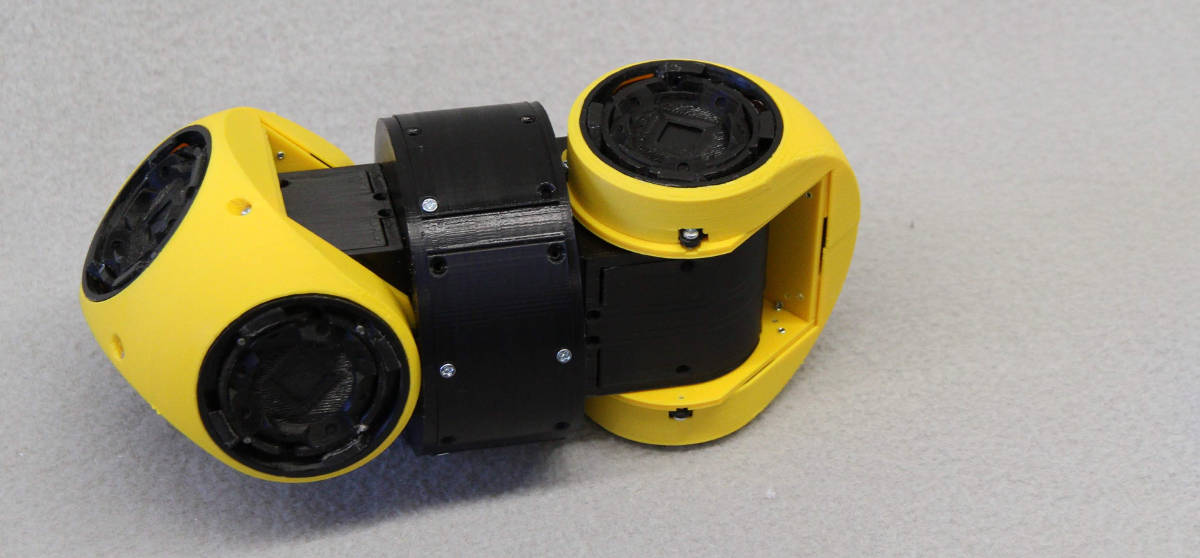
\includegraphics[width=0.6\textwidth]{pictures/module.jpg}
    \caption[Fotografia modulu]{Fotografia modulu \cite{rofiWeb}.}
    \label{fig:module}
\end{figure}

Každý z modulov sa skladá z dvoch častí (\textit{side A} a \textit{side B}). Každá z nich sa delí na dve časti označené ako \textit{body} a \textit{shoe} (viď obrázok \ref{fig:module_parts}). 

\begin{figure}[hbt!]
    \centering
    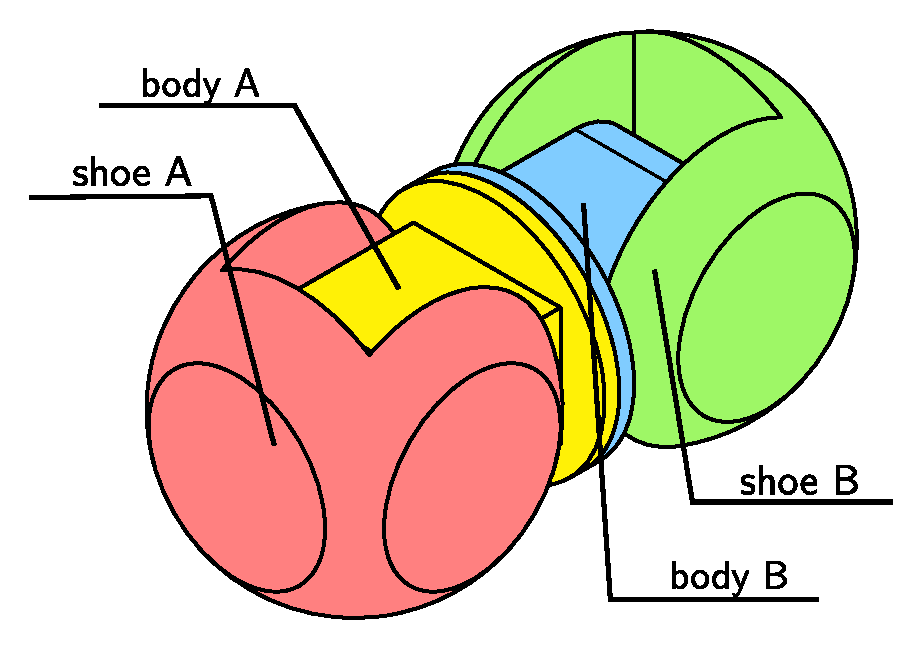
\includegraphics[width=0.6\textwidth]{pictures/module_parts.pdf}
    \caption[Časti modulu]{Schéma častí modulu \cite{mrazekMasterThesis}.}
    \label{fig:module_parts}
\end{figure}

Moduly majú schopnosť pohybovať sa, a to vďaka až trom stupňom voľnosti. Prvé dva z nich umožňujú pohybovať so shoe časťou modulu. Konkrétne ide o pohyb okolo osí označovaných ako $\alpha$ a $\beta$  o uhol v rozsahu $\interval[{-90\degree, 90\degree}]$. Posledným stupňom voľnosti je pohyb okolo osi označovanej ako $\gamma$. Tento pohyb umožňuje otáčaním meniť vzájomnú polohu body častí modulu a jeho rozsah je $\interval({-180\degree, 180\degree}]$. 

\begin{figure}[hbt!]
    \centering
    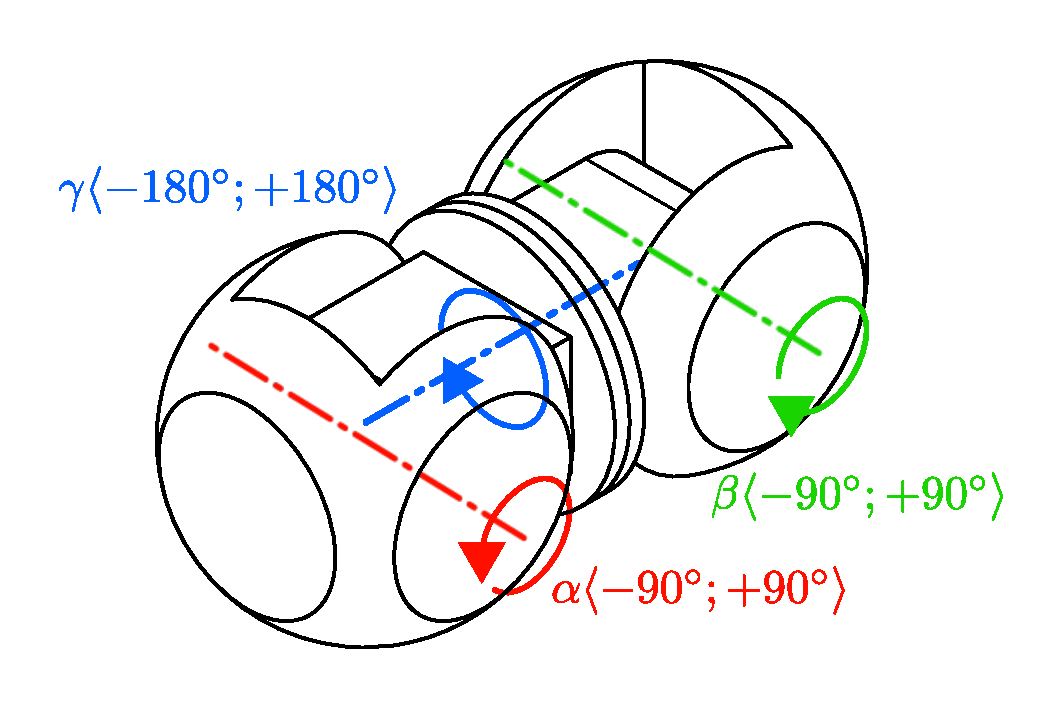
\includegraphics[width=0.6\textwidth]{pictures/module_angles.pdf}
    \caption[Stupne voľnosti modulu]{Schéma stupňov voľnosti modulu a smerov otáčania \cite{mrazekMasterThesis}.}
    \label{fig:module_angle}
\end{figure}

Ako bolo spomenuté vyššie, tak každý modul má schopnosť pripojiť sa k iným modulom (a vytvoriť tak RoFIbotov) alebo k pasívnym prvkom pomocou \textit{dock}ov. Dockovací systém platformy RoFI je navrhnutý ako tzv. \textit{genderless}, čo umožňuje vzájomné spojenie ľubovoľných dvoch dockov. 

\begin{figure}[hbt!]
    \centering
    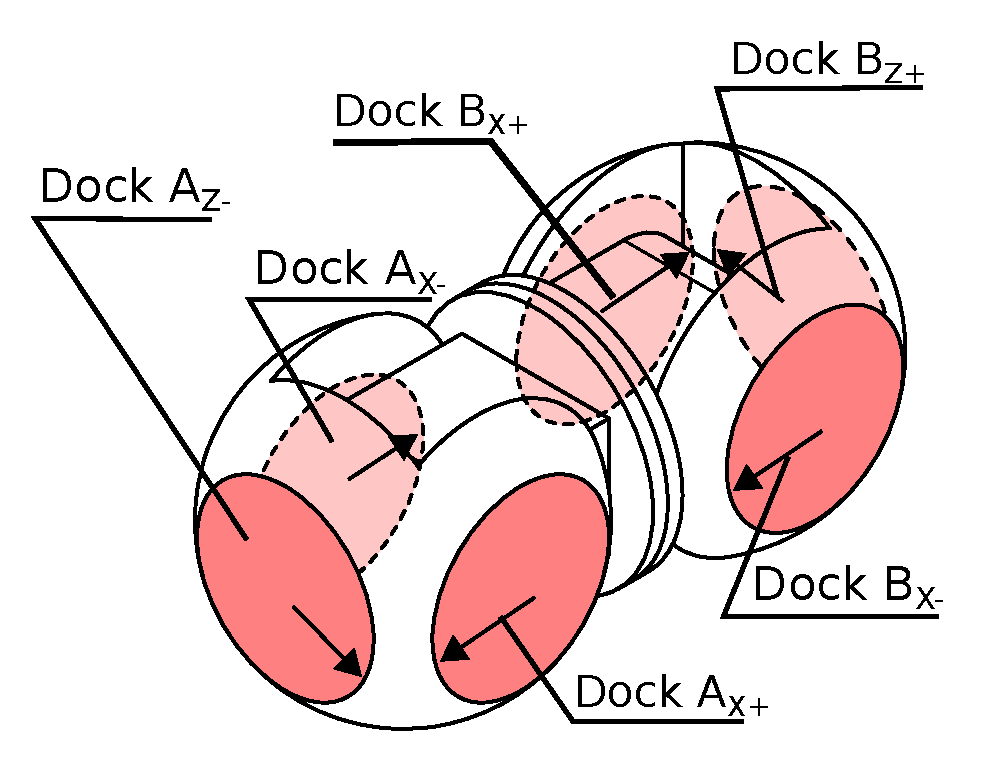
\includegraphics[width=0.6\textwidth]{pictures/dock_desc.pdf}
    \caption[Docky modulu]{Schéma umiestnení dockov na module a ich označenia. Šípky na dockoch znázorňujú orientačné vektory \cite{mrazekMasterThesis}.}
    \label{fig:dock_desc}
\end{figure}

Každý modul obsahuje práve šesť dockov, ktoré sú rozmiestnené po tri na každej shoe časti modulu. Dock je okrem svojej polohy na module definovaný aj orientačným vektorom (viď obrázok \ref{fig:dock_desc}). 

Prepojenie je definované vzájomnou polohou orientačných vektorov dockov spojenia. Konštrukcia dockov dovoľuje ich prepojenie až v štyroch rôznych polohách. 

Vzájomná poloha orientačných vektorov dockov môže byť postupne $0\degree$, $90\degree$, $180\degree$ alebo $270\degree$ a tieto prepojenia sa označujú v tomto poradí ako \textit{North}, \textit{East}, \textit{South} a \textit{West} (viď obrázok \ref{fig:dock_orientation}). 

\begin{figure}[hbt!]
    \centering
    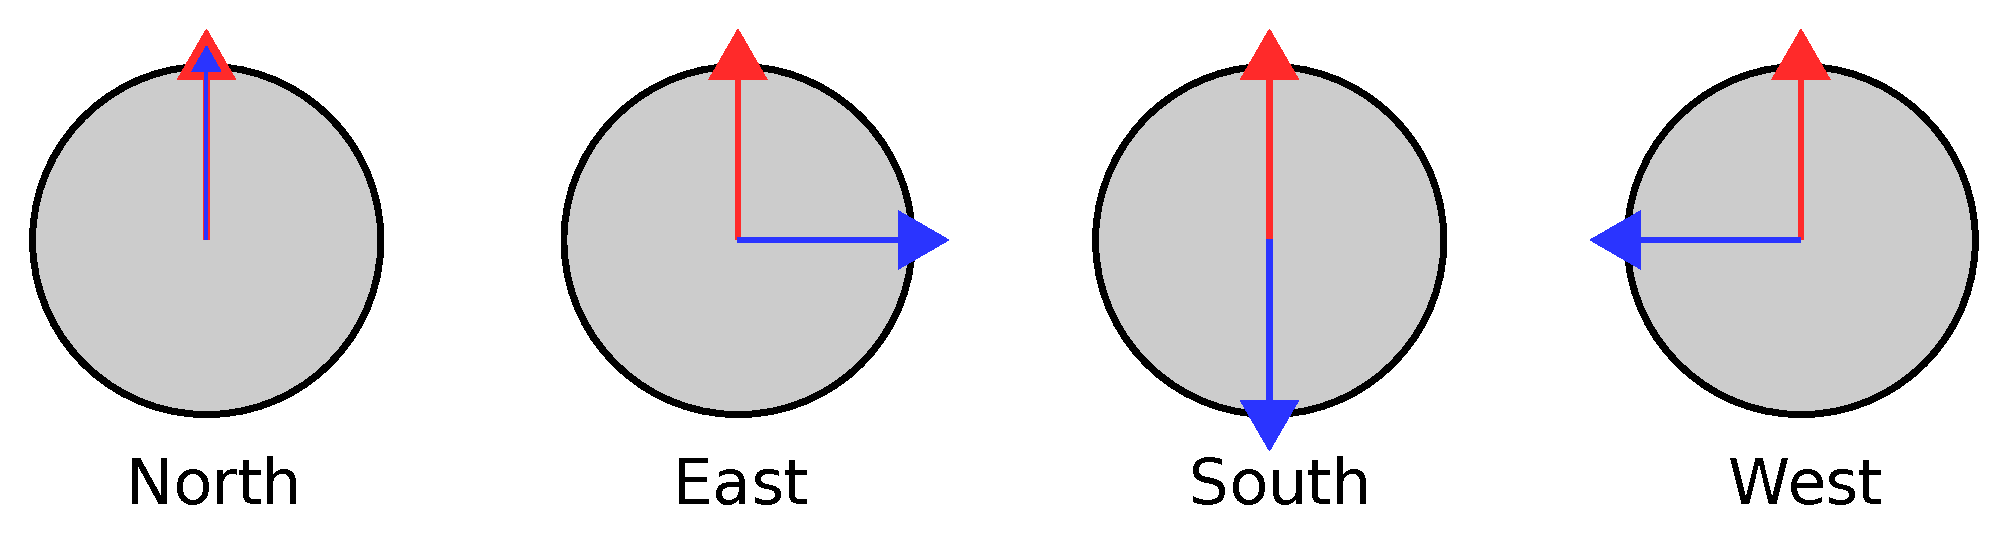
\includegraphics[width=0.6\textwidth]{pictures/dock_orientation.pdf}
    \caption[Poloha prepojenia dockov modulu]{Schéma vzájomnej polohy orientačných vektorov spojených dockov modulov. Červenou je označený dock modulu, z ktorého perspektívy spojenie označujeme. Modrá šípka je orientačný vektor druhého modulu. Poznámka: nezáleží na výbere docku, z ktorého perspektívy spojenie sledujeme \cite{mrazekMasterThesis}.}
    \label{fig:dock_orientation}
\end{figure}

\section{Popis RoFIbota}
\label{sec:rofibotSpec}
Vzájomné prepojenie modulov pomocou dockov vytvára RoFIbotov. Parametre RoFIbota, ktoré ho definujú, sa dajú rozdeliť do dvoch kategórií:   
\begin{enumerate}
    \item tvar RoFIbota vzhľadom na jeho vnútornú štruktúru: 
    \begin{itemize}[topsep=-5pt]
        \item množina modulov RoFIbota, 
        \item množina prepojení (hrán) modulov; 
    \end{itemize}
    \item poloha RoFIbota vzhľadom k okolitému svetu: 
    \begin{itemize}[topsep=-5pt]
        \item natočenie celého RoFIbota vzhľadom na okolie, 
        \item umiestnenie RoFIbota do priestoru.  
    \end{itemize}
\end{enumerate}

\textit{Konfigurácia} RoFIbota je tvar RoFIbota vzhľadom na jeho vnútornú štruktúru, teda množina modulov a ich prepojení. Každý modul v konfigurácii RoFIbota je definovaný jedinečným identifikátorom modulu a hodnotami všetkých troch stupňov voľnosti modulu. 

Jednotlivé hrany (prepojenia) v konfigurácii RoFIbota sú definované identifikátormi spojených modulov a presným popisom dockov, ktorými sú prepojené, a vzájomnou polohou spojených dockov. 

Formálne značenie všetkých parametrov konfigurácie a ich rozsahy sú zavedené v kapitole \ref{sec:formalSpec}. 

\textit{Rekonfigurácia} RoFIbota je postupnosť validných krokov (ich formálna definícia sa nachádza v kapitole \ref{sec:formalRecfg}), ktorá umožní zmeniť počiatočnú konfiguráciu RoFIbota na cieľovú konfiguráciu RoFIbota. 
% ------------------------------------------------------ 1 ------------------------------------------------------






% ------------------------------------------------------ 2 ------------------------------------------------------
\chapter{Distribuovaná rekonfigurácia RoFIbotov}
\section{Formálna špecifikácia komponent}
\label{sec:formalSpec}
Fyzický stav modulu a konfigurácie RoFIbota je nutné popísať z formálneho hľadiska. Na základe tohto popisu je následne definovaná aj rekonfigurácia RoFIbota. 

\subsection{Modul}
\label{sec:formalSpecModul}
V prvom rade je nutné definovať \textit{stav modulu}, ktorý je tvorený nasledujúcimi údajmi: 
\begin{itemize}
    \item \textit{id} -- unikátny identifikátor modulu, 
    \item $\alpha$ -- uhol otočenia shoe A voči body A v rozsahu $\interval[{-90\degree, 90\degree}]$,
    \item $\beta$ -- uhol otočenia shoe B voči body B v rozsahu $\interval[{-90\degree, 90\degree}]$,
    \item $\gamma$ -- uhol otočenia body A voči body B v rozsahu $\interval({-180\degree, 180\degree}]$,
    \item sedmice o každom prepojení, ktoré daný modul má. 
\end{itemize} 

Ako už bolo popísané v kapitole \ref{sec:moduleSpec}, tak spojenie definujú docky, ktorými sú moduly spojené, a ich vzájomná poloha. Formálne ide o nasledujúcu sedmicu: 
\begin{itemize}
    \item \textit{id1} -- unikátny identifikátor prvého modulu, 
    \item \textit{side1} -- strana prvého modulu, ktorou je spojený s druhým modulom, 
    \item \textit{dock1} -- dock prvého modulu, ktorý sa podieľa na prepojení,
    \item \textit{ori} -- orientácia spojených dockov,
    \item \textit{dock2} -- dock druhého modulu, ktorý sa podieľa na prepojení,
    \item \textit{side2} -- strana druhého modulu, ktorou je spojený s prvým modulom, 
    \item \textit{id2} -- unikátny identifikátor druhého modulu. 
\end{itemize}
Zároveň platí, že tieto hodnoty sú z množín: $side1, side2 \in \{A, B\}$; $dock1, dock2 \in \{X+, X-, Z-\}$; $ori \in \{N, E, S, W\}$.

\subsection{Konfigurácia}
\label{sec:formalSpecCfg}
Moduly sa spájajú do RoFIbotov a je nutné definovať si validitu konfigurácie. Konfigurácia RoFIbota je \textit{validná}, ak: 
\begin{itemize}
    \item každé prepojenie je vzájomné,
    \item každý dock každého modulu sa podieľa na maximálne jednom prepojení, 
    \item všetky definované prepojenia je možné fyzicky vytvoriť, 
    \item nesmie dochádzať k žiadnej fyzickej kolízii modulov. 
\end{itemize}
Formálny popis výpočtu kolízií v konfigurácii RoFIbota je podrobnejšie popísaný v diplomovej práci \textit{Motion Planning for the RoFI Platform} \cite{vozarovaMasterThesis}. 

Keďže komunikácia medzi modulmi môže prebiehať po fyzickom spojení pomocou dockov, ale aj bezdrôtovo, tak si zadefinujeme spojitosť RoFIbota. 

RoFIbot je \textit{spojitý}, ak medzi akýmikoľvek jeho dvomi modulmi existuje cesta tvorená modulmi a prepojeniami. To značí, že komunikácia medzi akýmikoľvek dvomi modulmi spojitého RoFIbota môže prebiehať výhradne fyzickými spojeniami (viď príklad spojitej a nespojitej konfigurácie na obrázku \ref{fig:exampleCfg}). 

\begin{figure}[hbt!]
    \centering
    \begin{subfigure}[b]{0.49\textwidth}
        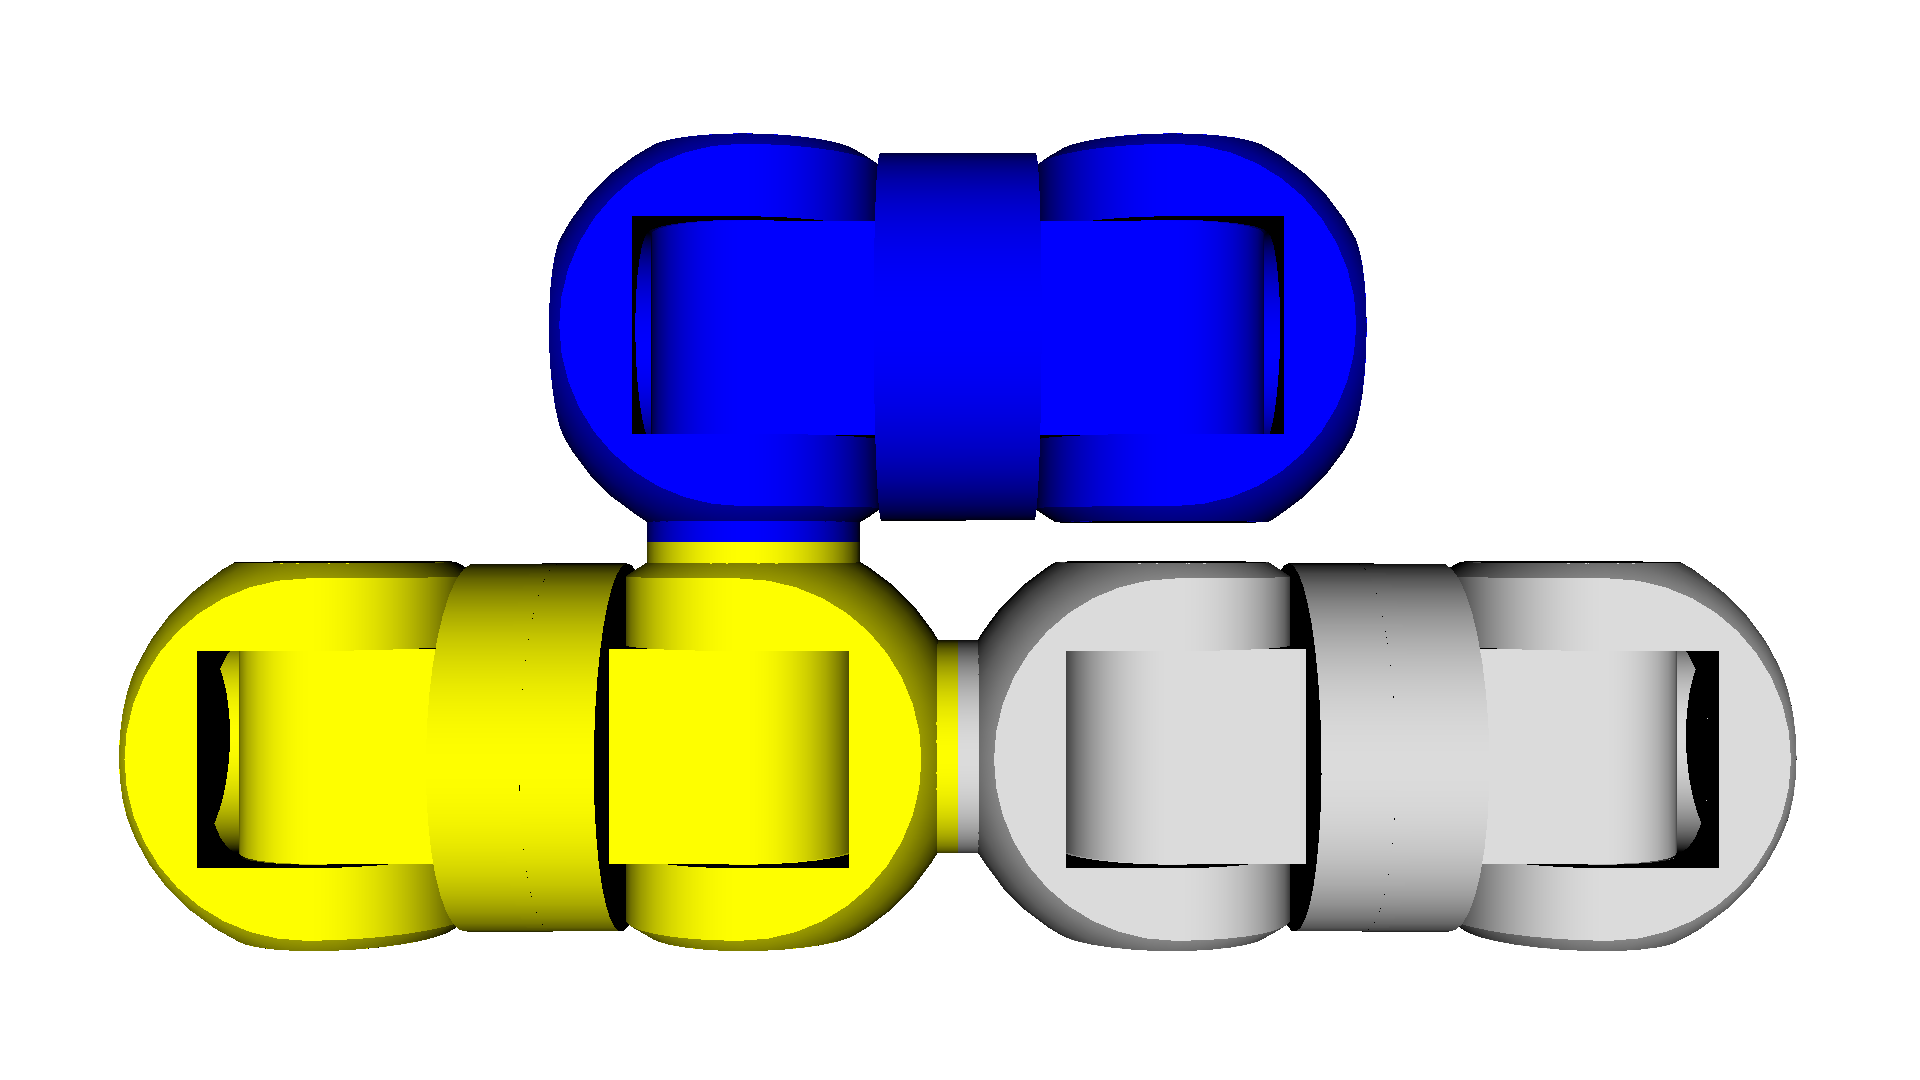
\includegraphics[width=\textwidth]{pictures/connected_rofibot.png}
        \caption[Spojitá konfigurácia.]{Spojitá konfigurácia}
        \label{fig:connectCfg}
    \end{subfigure}
    \begin{subfigure}[b]{0.49\textwidth}
        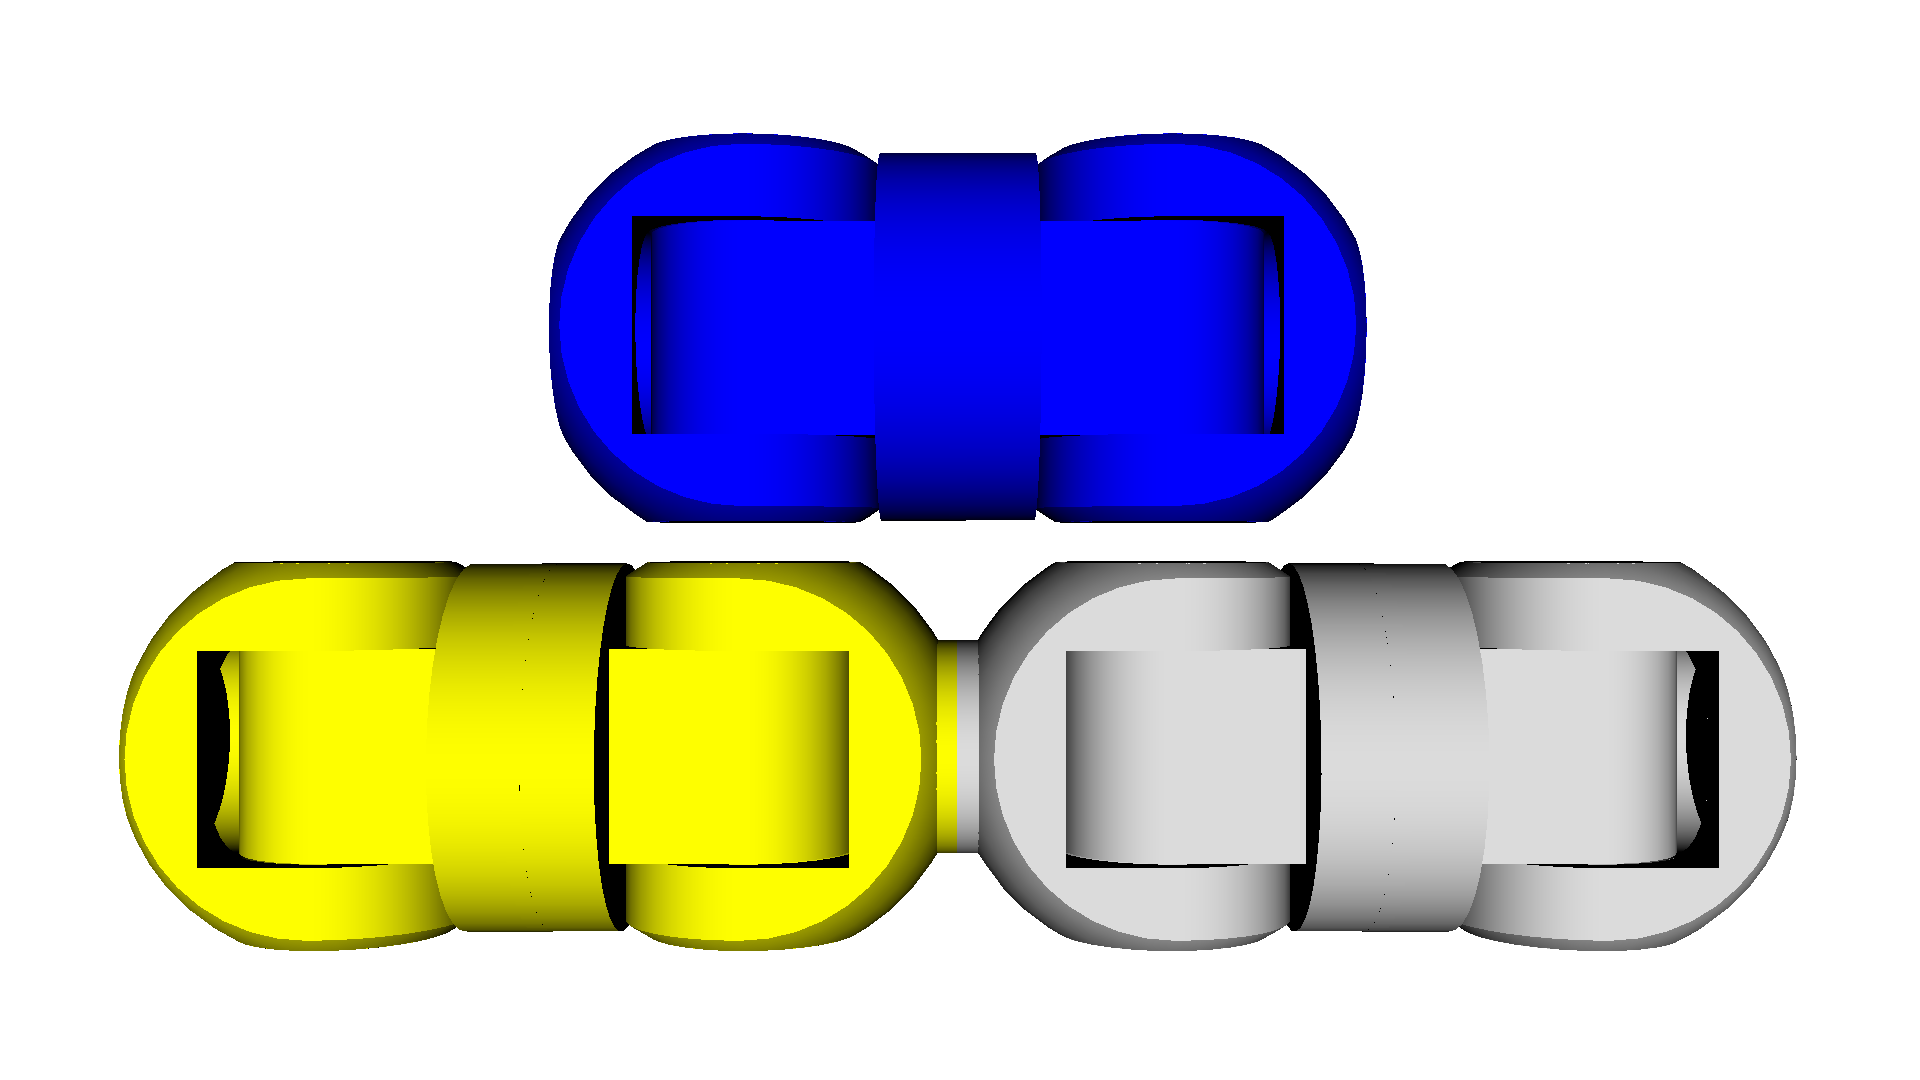
\includegraphics[width=\textwidth]{pictures/disconnected_rofibot.png}
        \caption[Nespojitá konfigurácia.]{Nespojitá konfigurácia}
        \label{fig:disconnectCfg}
    \end{subfigure}
    \caption[Príklad konfigurácie]{Príklad spojitej a nespojitej konfigurácie.}
    \label{fig:exampleCfg}
\end{figure}

Predpokladá sa, že každý modul je definovaný validne. To znamená, že údaje sú z popísaných rozsahov a množín. Každá hrana je definovaná pre oba prepojené moduly, a to v rovnakom tvare. Zároveň platí, že konfigurácia RoFIbota, ktorú popisujú dané stavy modulov, je spojitá a validná. 

\section{Formálna špecifikácia rekonfigurácie RoFIbota}
\label{sec:formalRecfg}
Atomickou zmenou v konfigurácii RoFIbota je \textit{akcia}, ktorá môže byť dvoch druhov. 

Prvým typom akcií je \textit{akcia rotácie}, ktorá sa deje na jednom z modulov RoFIbota a ide o zmenu jedného z parametrov $\alpha$, $\beta$ alebo $\gamma$. Je definovaná nasledovnými parametrami: 
\begin{itemize}
    \item \textit{id} -- id modulu, ktorý mení jeden z uhlov, 
    \item \textit{joint} -- identifikácia stupňa voľnosti; $joint \in \{\alpha, \beta, \gamma\}$, 
    \item \textit{angle} -- orientovaný uhol, o ktorý sa daný joint bude otáčať. 
\end{itemize}

Druhý typ akcie je \textit{akcia prepojenia}, ktorá definuje spojenie alebo rozpojenie dvoch modulov. Je definovaná nasledujúcimi parametrami: 
\begin{itemize}
    \item \textit{add} -- príznak, či ide o spojenie alebo rozpojenie,
    \item \textit{edge} -- popis hrany, ktorá buď vznikne alebo zanikne (sedmica definovaná v kapitole \ref{sec:moduleSpec}). 
\end{itemize}

Nie každú akciu je možné aplikovať na akúkoľvek konfiguráciu RoFIbota. \textit{Validná akcia} je akcia, ktorá spĺňa aj nasledujúce podmienky:
\begin{itemize}
    \item akcia rotácie: nesmie dôjsť ku kolízii s inými modulmi (viď obrázok \ref{fig:rotationExample}), 
    \item akcia prepojenia: docky, ktoré sa majú prepojiť, musia byť fyzicky schopné prepojenia (viď obrázok \ref{fig:reconnectionExample}). 
\end{itemize}

\begin{figure}[hbt!]
    \centering
    \begin{subfigure}[b]{\textwidth}
        \centering
        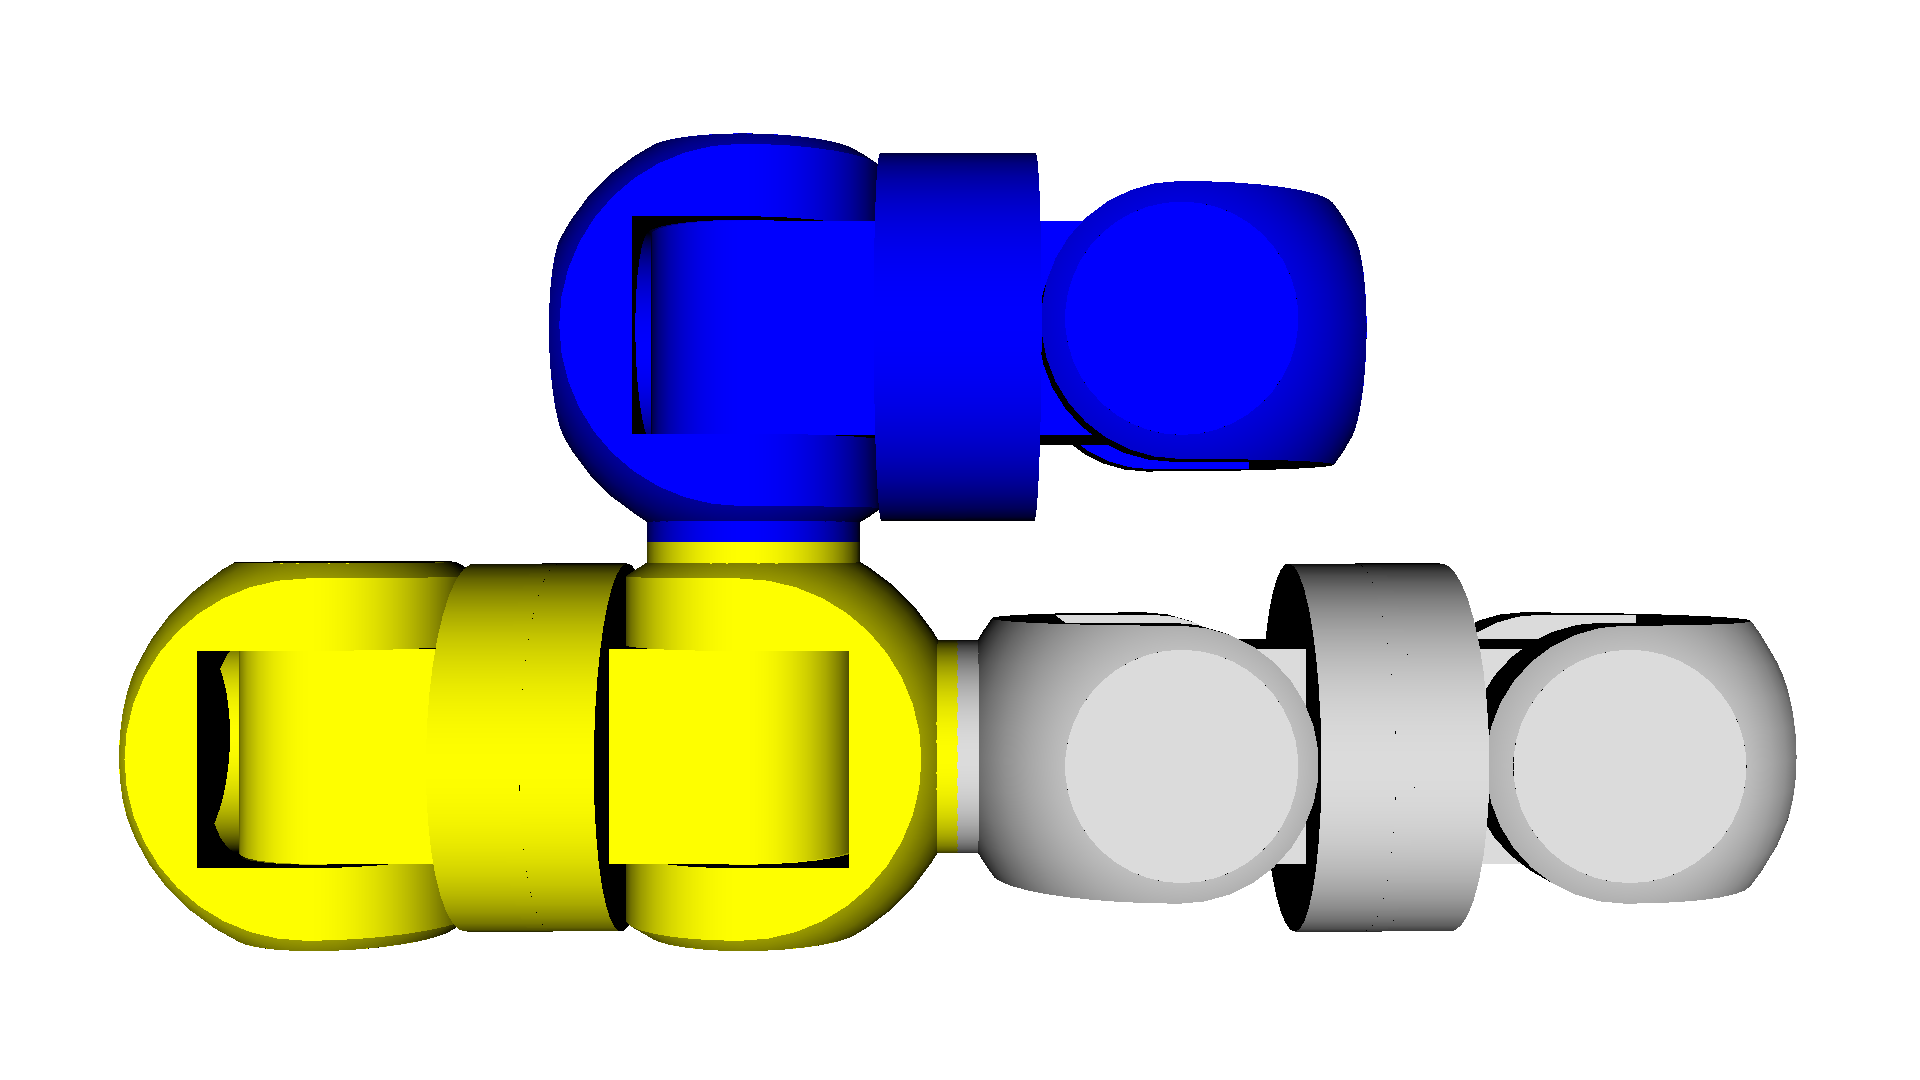
\includegraphics[width=0.47\textwidth]{pictures/rotation_example.png}
        \caption[Pred rotáciou]{Príklad konfigurácie pred rotáciou.}
    \end{subfigure}

    \begin{subfigure}[b]{0.47\textwidth}
        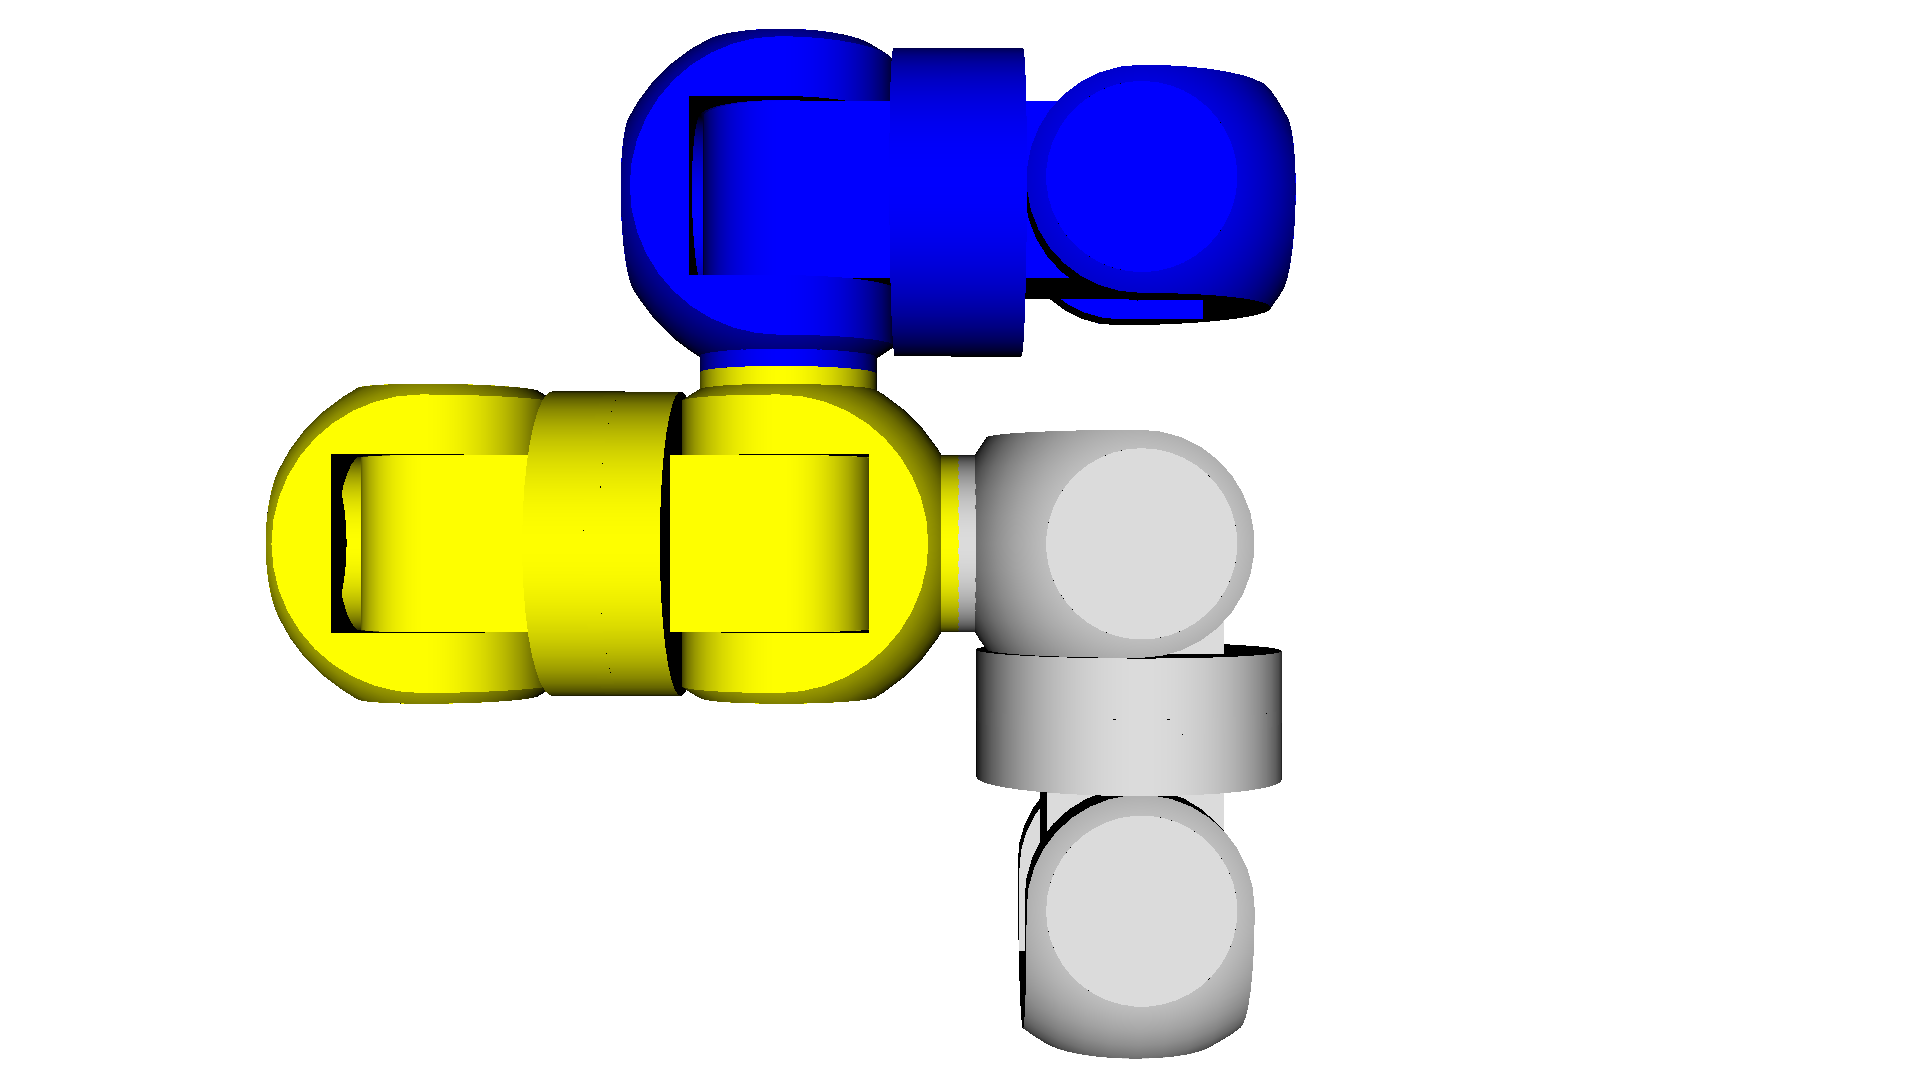
\includegraphics[width=\textwidth]{pictures/rotation_example_correct.png}
        \caption[Validná rotácia]{Validná rotácia modulu.}
    \end{subfigure}
    \begin{subfigure}[b]{0.47\textwidth}
        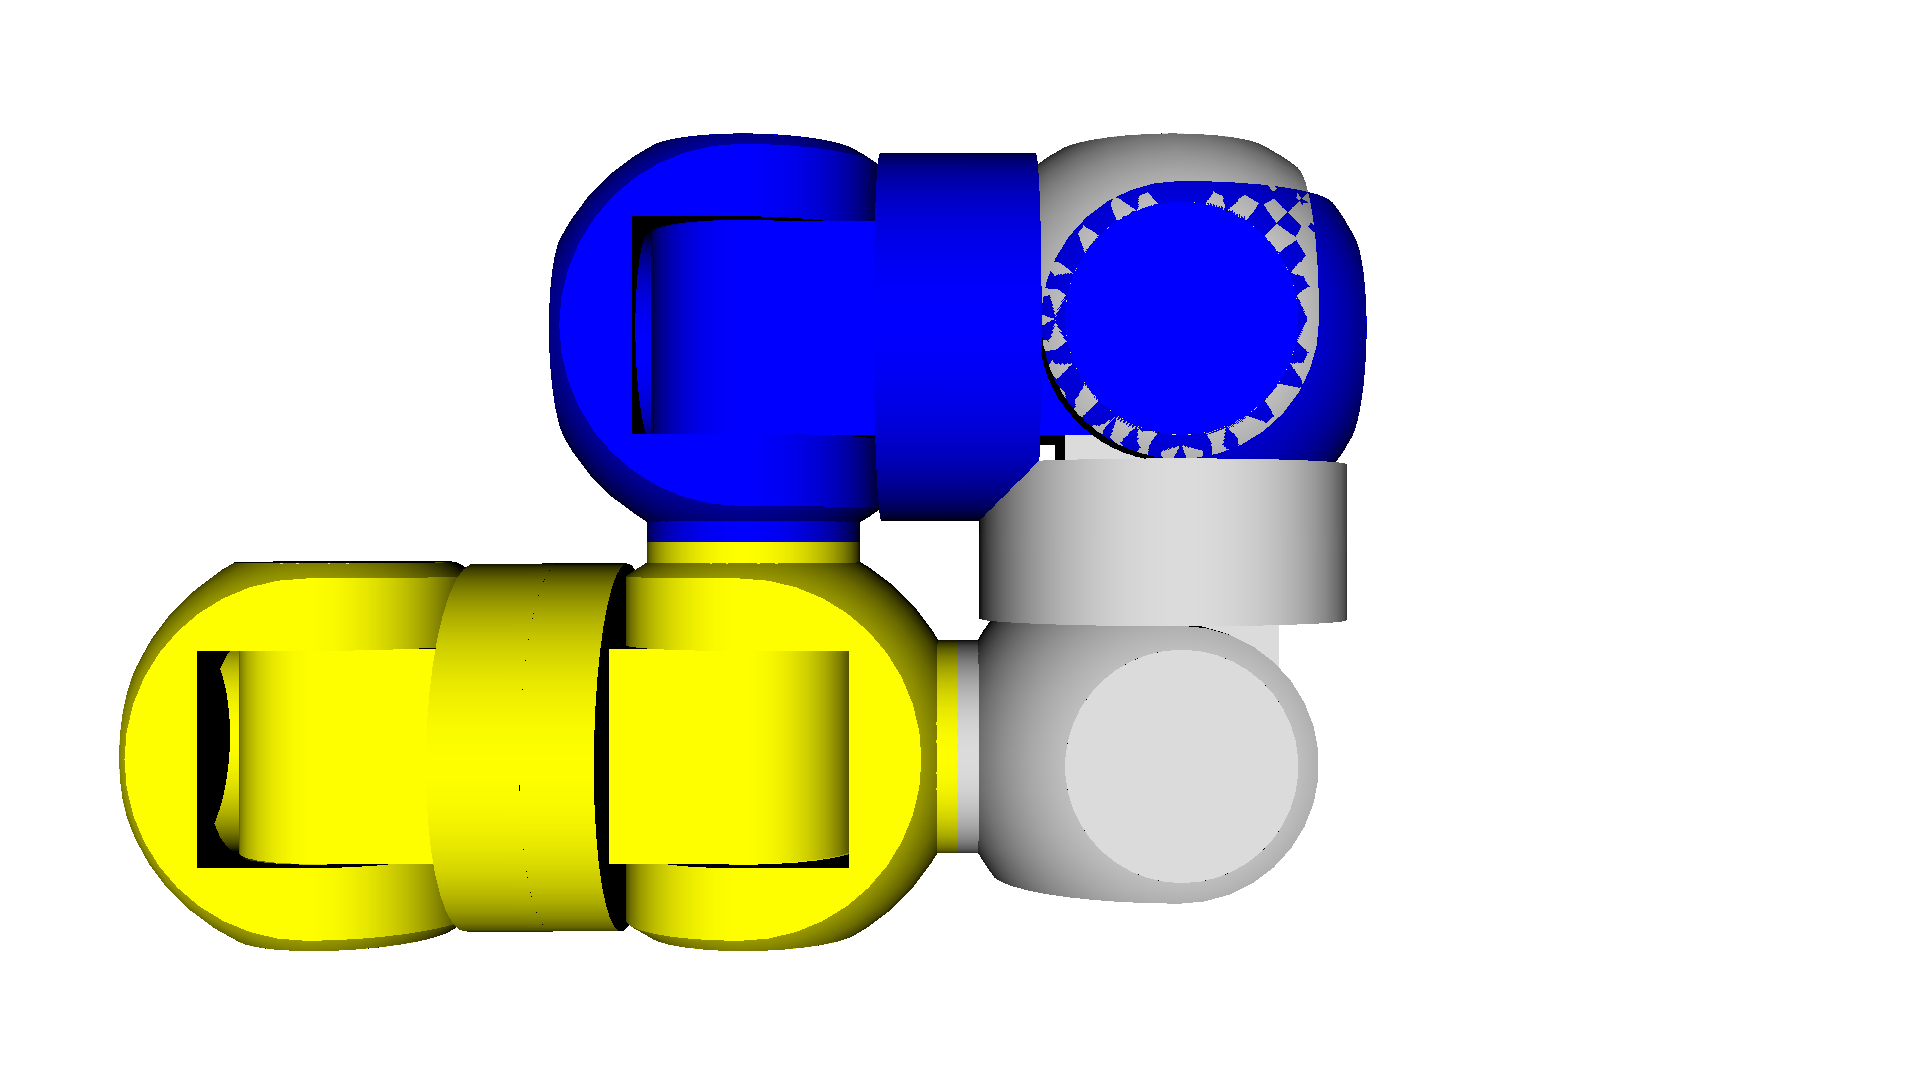
\includegraphics[width=\textwidth]{pictures/rotation_example_wrong.png}
        \caption[Nevalidná rotácia]{Nevalidná rotácia modulu.}
    \end{subfigure}
    \caption[Príklad akcie rotácie]{Príklad akcie rotácie (rotácia bieleho modulu o $90\degree$ uhla $\gamma$).}
    \label{fig:rotationExample}
\end{figure}

\begin{figure}[hbt!]
    \centering
    \begin{subfigure}[b]{\textwidth}
        \centering
        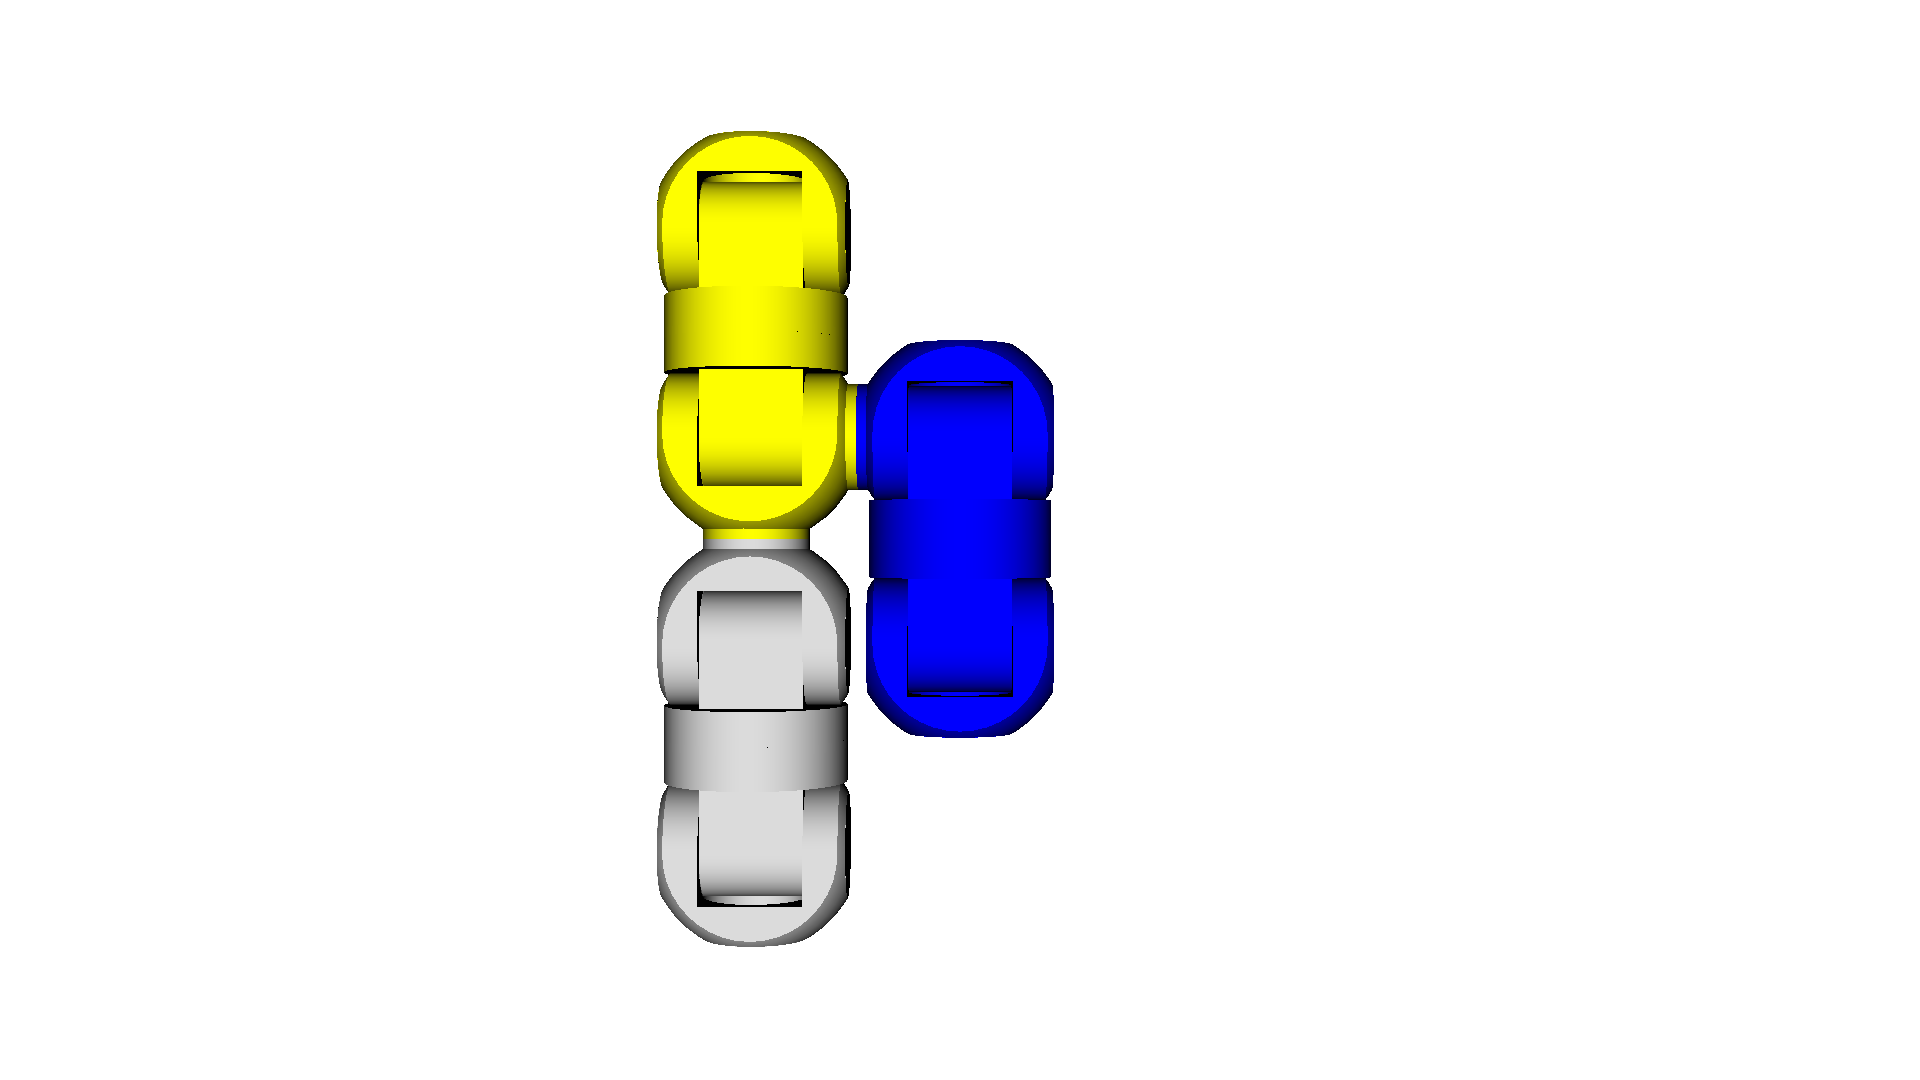
\includegraphics[width=0.8\textwidth]{pictures/reconnection_example.png}
        \caption[Pred prepojením]{Príklad konfigurácie pred vytvorením spojenia.}
    \end{subfigure}

    \begin{subfigure}[b]{0.47\textwidth}
        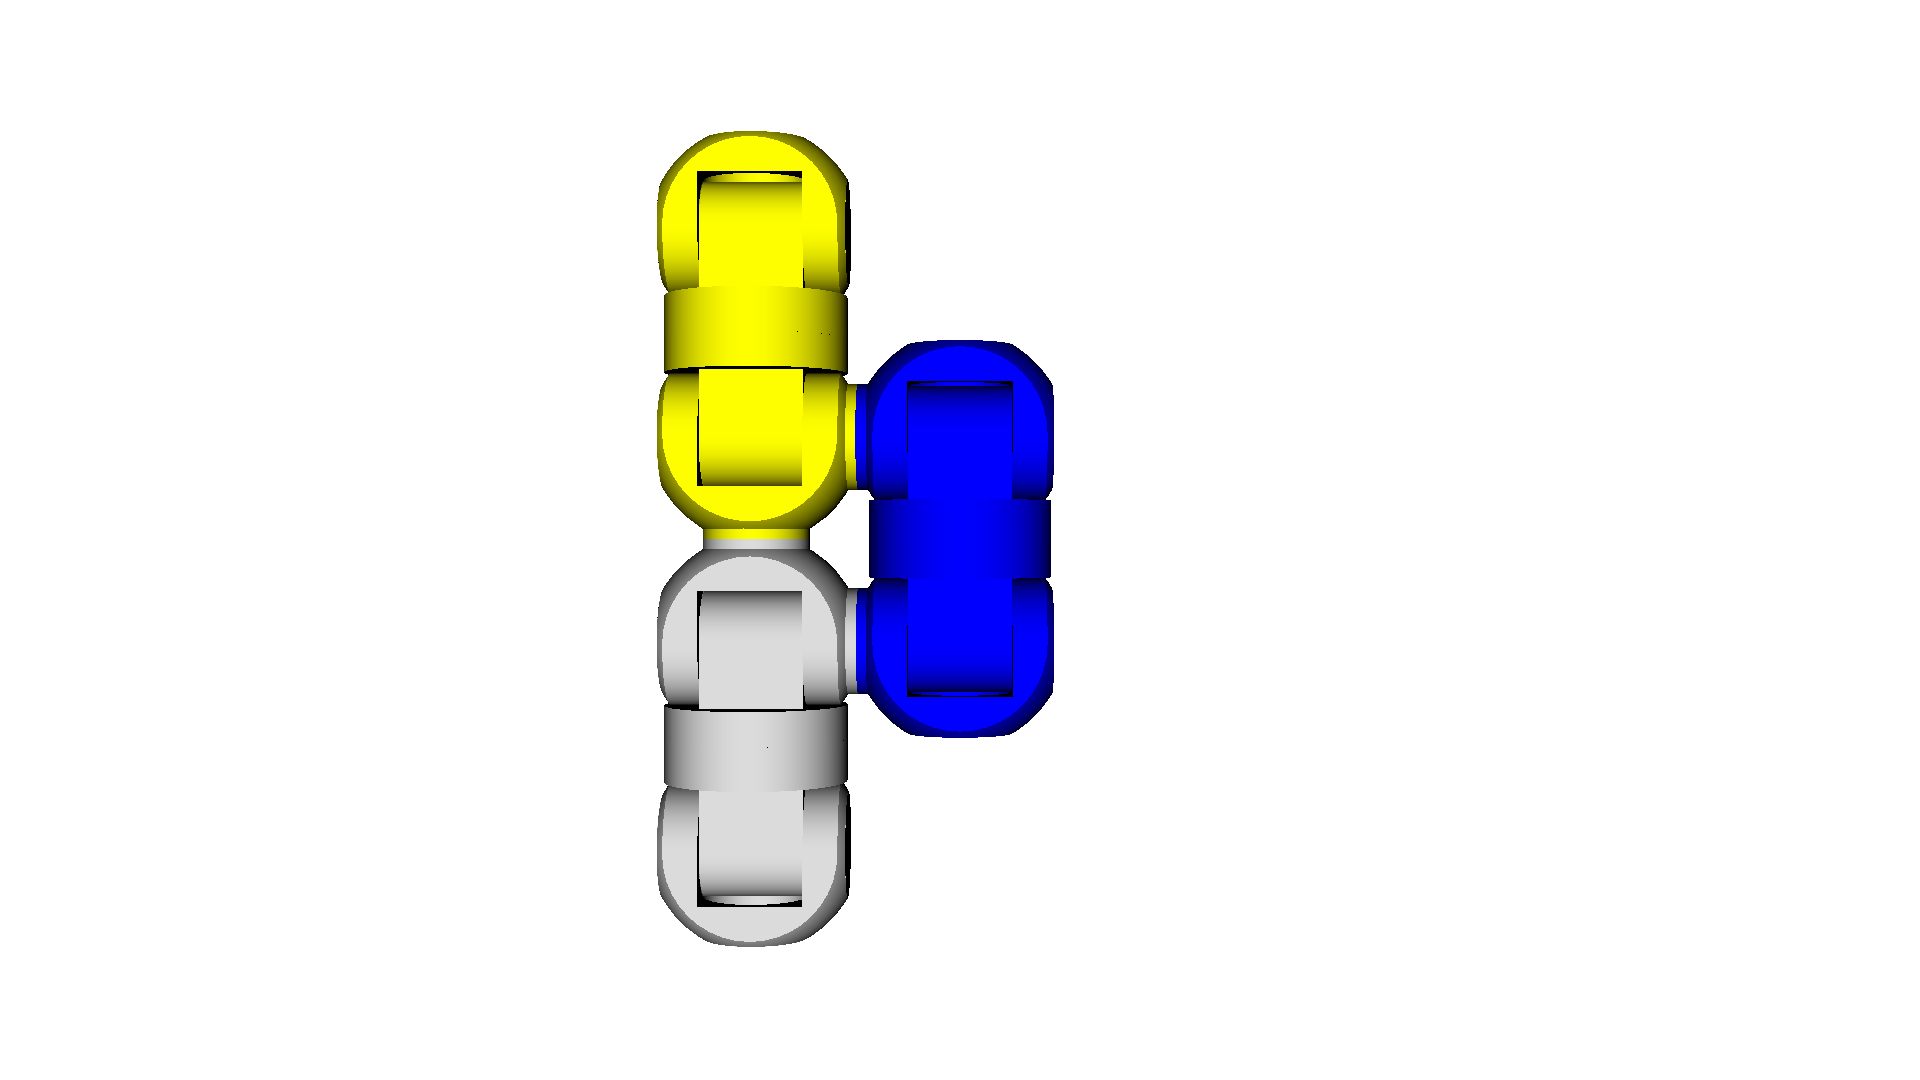
\includegraphics[width=\textwidth]{pictures/reconnection_example_correct.png}
        \caption[Validné spojenie]{Validné spojenie modulov \\(obidva sa podieľajú na spojení).}
    \end{subfigure}
    \begin{subfigure}[b]{0.47\textwidth}
        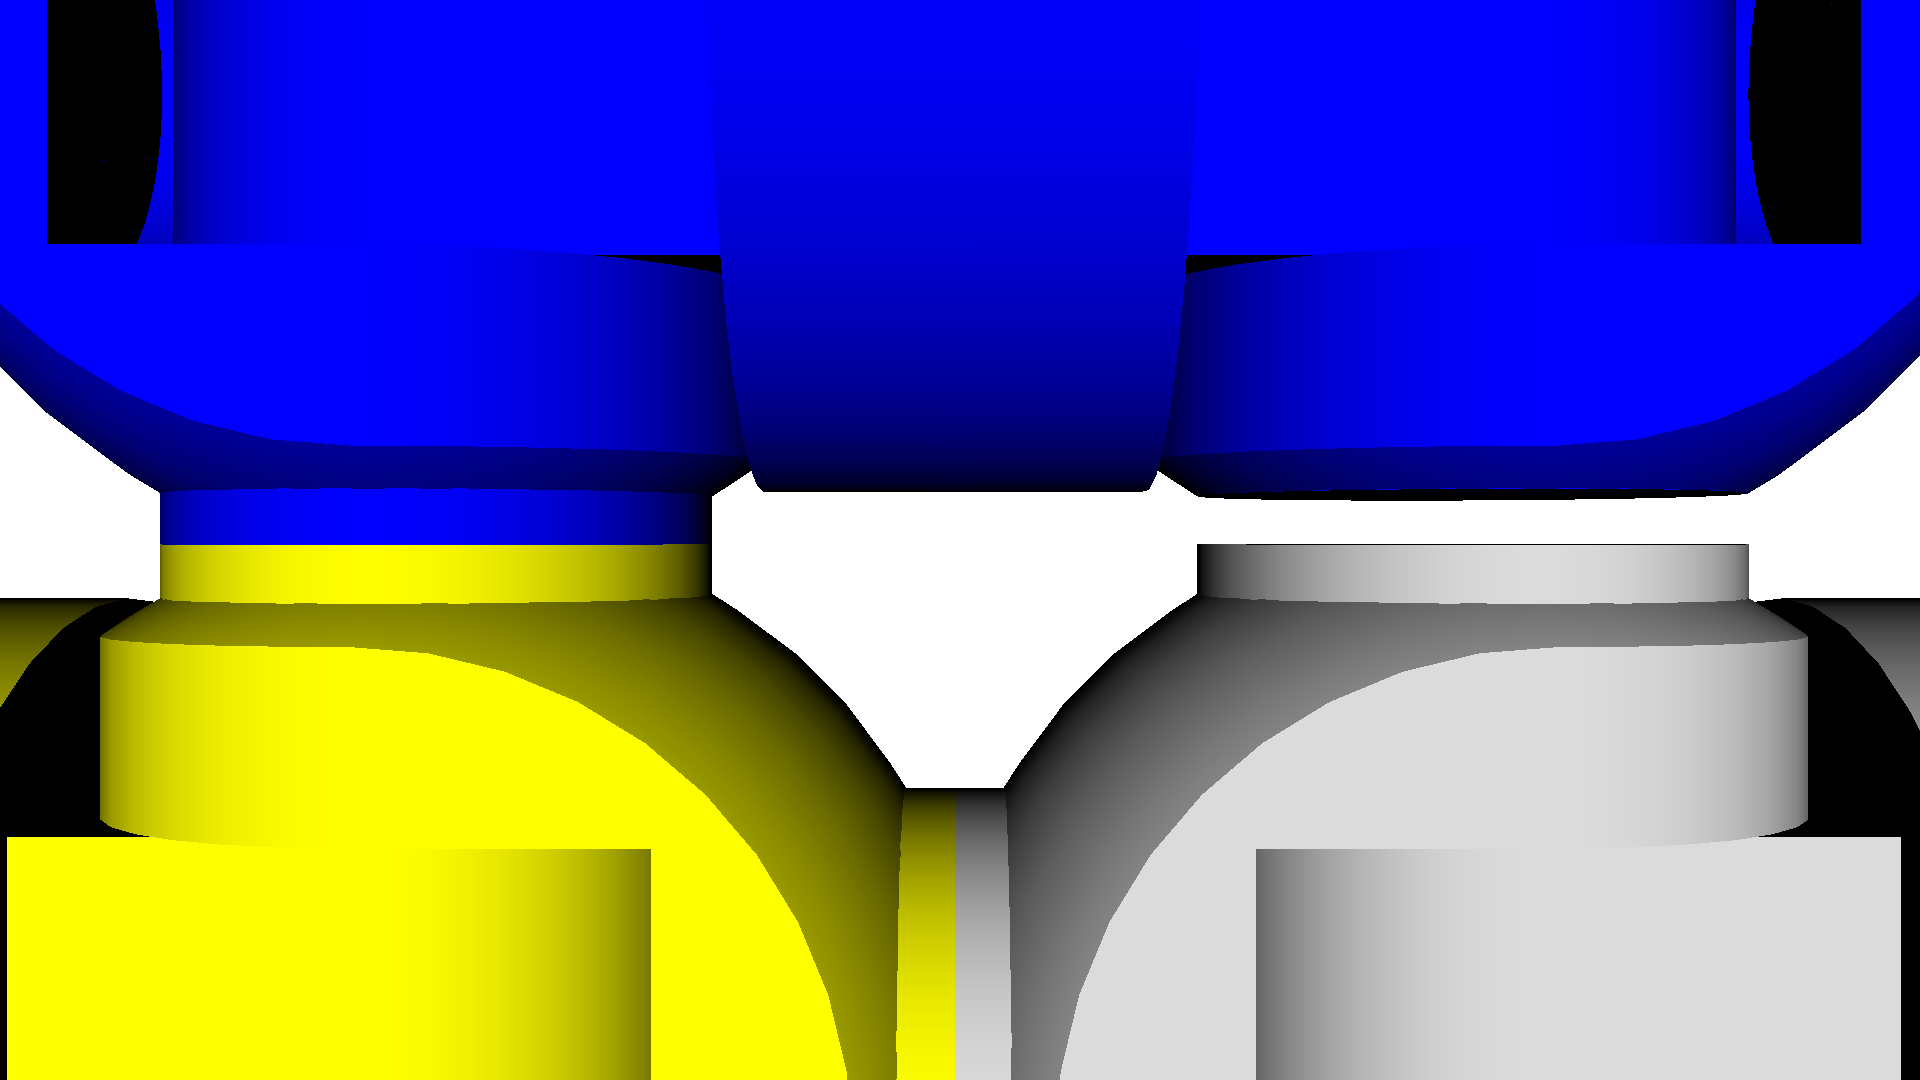
\includegraphics[width=\textwidth]{pictures/reconnection_example_wrong.png}
        \caption[Nevalidné prepojenie]{Nevalidné spojenie modulov \\(modrý sa nepodieľa na spojení).}
    \end{subfigure}
    \caption[Príklad akcie prepojenia]{Príklad akcie prepojenia (medzi bielym a modrým modulom).}
    \label{fig:reconnectionExample}
\end{figure}

% {0, 0, 136},
% {0, 0, 255},
% {119, 119, 255},
% {220, 220, 220},
% {255, 255, 136},
% {255, 255, 0},
% {119, 119, 0}};

\textit{Krok rekonfigurácie} je definovaný ako množina validných akcií. Poradie vykonávania akcií v jednom krku rekonfigurácie nie je presne definované (prebiehajú zároveň, ale synchronizácia nikdy nie je úplne presná). 

Pre spojitých RoFIbotov musí platiť, že ak je konfigurácia pred krokom spojitá a validná, tak aj počas vykonávania kroku a po jeho vykonaní musí byť konfigurácia spojitá a validná. \textit{Validný krok} je krok rekonfigurácie taký, že konfigurácia je spojitá aj v prípade, ak sa vykonajú iba všetky rozpojenia a žiadne iné akcie. 

Rekonfigurácia RoFIbota je definovaná ako postupnosť validných krokov. 

\section{Popis problému}
\label{sec:problemDesc}
Cieľom tejto práce je navrhnúť a implementovať algoritmy na rekonfiguráciu RoFIbotov, ktoré spĺňajú podmienky popísané v tejto kapitole, a následne evaluovať výsledky. 

Diplomová práca \textit{Motion Planning for the RoFI Platform} \cite{vozarovaMasterThesis} popisuje rekonfiguráciu RoFIbotov z centralizovaného pohľadu. To znamená, že algoritmy na rekonfiguráciu majú úplnú znalosť počiatočnej a cieľovej konfigurácie RoFIbota. 

Platforma RoFI je však navrhnutá ako distribuovaný systém, kde najmenšou stavebnou jednotkou je modul. Zároveň je platforma navrhnutá tak, že RoFIbot nemá žiadnu centralizovanú logickú jednotku, ktorá by dokázala riadiť rekonfiguráciu. 

Navrhnuté algoritmy považujú modul za samostatnú entitu, ktorá na vstup dostane počiatočný a cieľový stav modulu, ktorý reprezentuje. Výstupom tejto entity je zoznam akcií, ktoré daný modul vykonal počas rekonfigurácie RoFIbota v jednom momente s prihliadnutím na validitu a spojitosť. V prípade, že sa RoFIbot nedokáže rekonfigurovať z počiatočnej konfigurácie do cieľovej, tak implementované algoritmy túto skutočnosť dokážu identifikovať. 

Samotný modul nepozná celú konfiguráciu RoFIbota (dokonca pri veľkých konfiguráciách by znalosť celej konfigurácie mohla zaberať veľa miesta v pamäti a nebola by potrebná). V tejto práci má každý modul znalosť výhradne o svojom stave, pričom každý ďalší údaj o stave iných modulov vie získať výhradne posielaním si správ so susednými modulmi. 

Implementované algoritmy sú iba simuláciou reálnych rekonfigurácií RoFIbotov, teda je možné zaviesť si obmedzujúce podmienky na svet, kde sa RoFIboti rekonfigurujú. 

Ako je popísané v kapitole \ref{sec:rofibotSpec}, tak konfigurácia RoFIbota je tvar RoFIbota vzhľadom na jeho vnútornú štruktúru. Teda pre účely tejto práce je zavedený predpoklad, že RoFIboti nemajú definované natočenie a umiestnenie do okolitého sveta. 

Každý RoFIbot vykonáva svoju rekonfiguráciu „vo vákuu“, bez fyzických obmedzení reálneho sveta (ako je napríklad podlaha, či iné prekážky). Pri rekonfigurácii nehrajú rolu ani fyzikálne zákony (napríklad gravitácia). Zároveň musí platiť, že počas celej rekonfigurácie musí byť RoFIbot vo validnej a spojitej konfigurácií. 

To značí, že RoFIbot nemusí mať žiadne vnímanie okolitého sveta. Jedinými prekážkami v pohyboch sú moduly samotné (ich poloha) a tú si entity vedia zistiť pomocou posielania si správ. 

\section{Popis algoritmov na rekonfiguráciu}
\label{sec:algoDesc}
\subsection{Centralizovane-distribuovaný algoritmus - //TODO premenovat}
\subsection{Distribuovaný algoritmus}

% ------------------------------------------------------ 2 ------------------------------------------------------



% ------------------------------------------------------ 3 ------------------------------------------------------

\chapter{Implementácia}
\label{sec:implementation}
Platforma RoFI, ako už bolo spomenuté v kapitole \ref{sec:platform}, je open-source projekt. Časť RoFILib\footnote{\url{https://github.com/paradise-fi/RoFI/tree/master/RoFILib}} sa zaoberá vývojom simulácií a vizualizácie, kde patrí aj implementačná časť tejto práce. 

RoFILib je knižnica naprogramovaná v jazyku C++. Táto knižnica poskytuje funkcie na simuláciu rekonfigurácie rôznymi algoritmami a z rôznych pohľadov na problém rekonfigurácie. V súčasnej dobe sú to algoritmy navrhnuté v rámci tejto práce a v diplomovej práci \textit{Motion Planning for the RoFI Platform} \cite{vozarovaMasterThesis}.

Knižnica zároveň poskytuje možnosť vizualizácie konfigurácií a rekonfigurácií RoFIbotov. Vizualizér vznikol ako bakalárska práca \textit{Vizualizace pro robotickou platformu RoFI} \cite{nausovaBachelorThesis} a dokáže produkovať obrázky konfigurácie alebo videá rekonfigurácie. Obrázky v tejto práci sú výstupom vizualizéru. 

\section{Technická špecifikácia a využité knižnice}
\label{sec:libraries}
Problémy majú nasledujúce vstupy a výstupy: Na vstupe sa nachádzajú dva súbory, ktoré popisujú počiatočnú a cieľovú konfiguráciu RoFIbota, ktorý sa má rekonfigurovať. Výstupom je súbor, ktorý obsahuje zoznam konfigurácií RoFIbota takých, ktoré vznikli po každom kroku rekonfigurácie. 

Podrobný popis vstupných a výstupných súborov sa nachádza v diplomovej práci \textit{Motion Planning for the RoFI Platform} \cite{vozarovaMasterThesis}. Tieto súbory sú zároveň kompatibilné s vizualizérom. 

Vstupné a výstupné súbory obsahujú celú konfiguráciu RoFIbota, ktorej celková znalosť na vstupe simulácie ľubovoľného modulu nie je pre túto prácu možná. Tým pádom z dôvodu kompatibility so zvyškom knižnice je implementovaný aj preprocessing a postprocessing, ktorý obaľuje implementované algoritmy. 

Algoritmy v tejto práci sú navrhnuté tak, aby každý modul RoFIbota fungoval ako samostatná entita. Komunikácia medzi entitami je možná výhradne pomocou správ. V softvéri fyzických modulov je implementovaný protokol MPI\footnote{Message Passing Interface}. 

Z týchto dôvodov je implementácia navrhnutých algoritmov v jazyku C++ s využitím knižnice OpenMPI \cite{openMPILibrary}. 

Knižnica OpenMPI umožňuje spustiť zadaný počet procesov s rovnakým programom a unikátnou identifikáciou pre každý z nich. Zároveň poskytuje komunikačnú vrstvu medzi zadanými procesmi (príkladom je posielanie správ medzi dvomi konkrétnymi procesmi, broadcast alebo all-to-all komunikácia). 

Simulácia v tejto práci prebieha tak, že každý modul je samostatný proces, ktorý dostane na vstup vstupné informácie (svoj počiatočný a cieľový stav). 

Spustený program následne dokáže pomocou posielania správ medzi procesmi vykonať validné akcie tak, aby sa každý modul rekonfiguroval z počiatočného stavu do cieľového stavu. 

Každú vykonanú akciu sú procesy schopné vhodným spôsobom zapísať do logu. Z logov je následne možné vytvoriť súbor kompatibilný s vizualizérom. 

Simulácia sa má čo najviac podobať fyzickému modelu rekonfigurácie RoFIbota. To znamená, že algoritmy využívajú iba minimálnu sadu funkcií a možností knižnice OpenMPI, a to tie, ktoré je možné využiť vo fyzických moduloch. Príkladom tohto obmedzenia je, že algoritmy nevyužívajú zdieľanú pamäť, lebo fyzické moduly nemajú žiadnu zdieľanú pamäť. 

% ------------------------------------------------------ 3 ------------------------------------------------------




% ------------------------------------------------------ 4 ------------------------------------------------------
\chapter{Experimentálne vyhodnotenie}
\section{Ukážkové rekonfigurácie}
Ukážkové konfigurácie a porovnanie rýchlostí ich výpočtov a prípadne rôznorodosti nájdených riešení

Odkazy na videá, obrázky, presné časy behov a rôznosť riešení. 
\section{Evaluácia výsledkov na vzorových príkladoch}
Porovnanie algoritmov z pohľadu časovej a priestorovej zložitosti

Popis, ktorý algoritmus a na aké konfigurácie a zmeny v rekonfiguráciách je viac vhodný

% ------------------------------------------------------ 4 ------------------------------------------------------


\chapter{Záver}
Rekapitulácia. 
Ako ďalej zlepšovať algoritmy a čo ešte pridávať a podobne. 

\printbibliography[heading=bibintoc] %% Print the bibliography.


\end{document}
